\documentclass[1p]{elsarticle_modified}
%\bibliographystyle{elsarticle-num}

%\usepackage[colorlinks]{hyperref}
%\usepackage{abbrmath_seonhwa} %\Abb, \Ascr, \Acal ,\Abf, \Afrak
\usepackage{amsfonts}
\usepackage{amssymb}
\usepackage{amsmath}
\usepackage{amsthm}
\usepackage{scalefnt}
\usepackage{amsbsy}
\usepackage{kotex}
\usepackage{caption}
\usepackage{subfig}
\usepackage{color}
\usepackage{graphicx}
\usepackage{xcolor} %% white, black, red, green, blue, cyan, magenta, yellow
\usepackage{float}
\usepackage{setspace}
\usepackage{hyperref}

\usepackage{tikz}
\usetikzlibrary{arrows}

\usepackage{multirow}
\usepackage{array} % fixed length table
\usepackage{hhline}

%%%%%%%%%%%%%%%%%%%%%
\makeatletter
\renewcommand*\env@matrix[1][\arraystretch]{%
	\edef\arraystretch{#1}%
	\hskip -\arraycolsep
	\let\@ifnextchar\new@ifnextchar
	\array{*\c@MaxMatrixCols c}}
\makeatother %https://tex.stackexchange.com/questions/14071/how-can-i-increase-the-line-spacing-in-a-matrix
%%%%%%%%%%%%%%%

\usepackage[normalem]{ulem}

\newcommand{\msout}[1]{\ifmmode\text{\sout{\ensuremath{#1}}}\else\sout{#1}\fi}
%SOURCE: \msout is \stkout macro in https://tex.stackexchange.com/questions/20609/strikeout-in-math-mode

\newcommand{\cancel}[1]{
	\ifmmode
	{\color{red}\msout{#1}}
	\else
	{\color{red}\sout{#1}}
	\fi
}

\newcommand{\add}[1]{
	{\color{blue}\uwave{#1}}
}

\newcommand{\replace}[2]{
	\ifmmode
	{\color{red}\msout{#1}}{\color{blue}\uwave{#2}}
	\else
	{\color{red}\sout{#1}}{\color{blue}\uwave{#2}}
	\fi
}

\newcommand{\Sol}{\mathcal{S}} %segment
\newcommand{\D}{D} %diagram
\newcommand{\A}{\mathcal{A}} %arc


%%%%%%%%%%%%%%%%%%%%%%%%%%%%%5 test

\def\sl{\operatorname{\textup{SL}}(2,\Cbb)}
\def\psl{\operatorname{\textup{PSL}}(2,\Cbb)}
\def\quan{\mkern 1mu \triangleright \mkern 1mu}

\theoremstyle{definition}
\newtheorem{thm}{Theorem}[section]
\newtheorem{prop}[thm]{Proposition}
\newtheorem{lem}[thm]{Lemma}
\newtheorem{ques}[thm]{Question}
\newtheorem{cor}[thm]{Corollary}
\newtheorem{defn}[thm]{Definition}
\newtheorem{exam}[thm]{Example}
\newtheorem{rmk}[thm]{Remark}
\newtheorem{alg}[thm]{Algorithm}

\newcommand{\I}{\sqrt{-1}}
\begin{document}

%\begin{frontmatter}
%
%\title{Boundary parabolic representations of knots up to 8 crossings}
%
%%% Group authors per affiliation:
%\author{Yunhi Cho} 
%\address{Department of Mathematics, University of Seoul, Seoul, Korea}
%\ead{yhcho@uos.ac.kr}
%
%
%\author{Seonhwa Kim} %\fnref{s_kim}}
%\address{Center for Geometry and Physics, Institute for Basic Science, Pohang, 37673, Korea}
%\ead{ryeona17@ibs.re.kr}
%
%\author{Hyuk Kim}
%\address{Department of Mathematical Sciences, Seoul National University, Seoul 08826, Korea}
%\ead{hyukkim@snu.ac.kr}
%
%\author{Seokbeom Yoon}
%\address{Department of Mathematical Sciences, Seoul National University, Seoul, 08826,  Korea}
%\ead{sbyoon15@snu.ac.kr}
%
%\begin{abstract}
%We find all boundary parabolic representation of knots up to 8 crossings.
%
%\end{abstract}
%\begin{keyword}
%    \MSC[2010] 57M25 
%\end{keyword}
%
%\end{frontmatter}

%\linenumbers
%\tableofcontents
%
\newcommand\colored[1]{\textcolor{white}{\rule[-0.35ex]{0.8em}{1.4ex}}\kern-0.8em\color{red} #1}%
%\newcommand\colored[1]{\textcolor{white}{ #1}\kern-2.17ex	\textcolor{white}{ #1}\kern-1.81ex	\textcolor{white}{ #1}\kern-2.15ex\color{red}#1	}

{\Large $\underline{11a_{179}~(K11a_{179})}$}

\setlength{\tabcolsep}{10pt}
\renewcommand{\arraystretch}{1.6}
\vspace{1cm}\begin{tabular}{m{100pt}>{\centering\arraybackslash}m{274pt}}
\multirow{5}{120pt}{
	\centering
	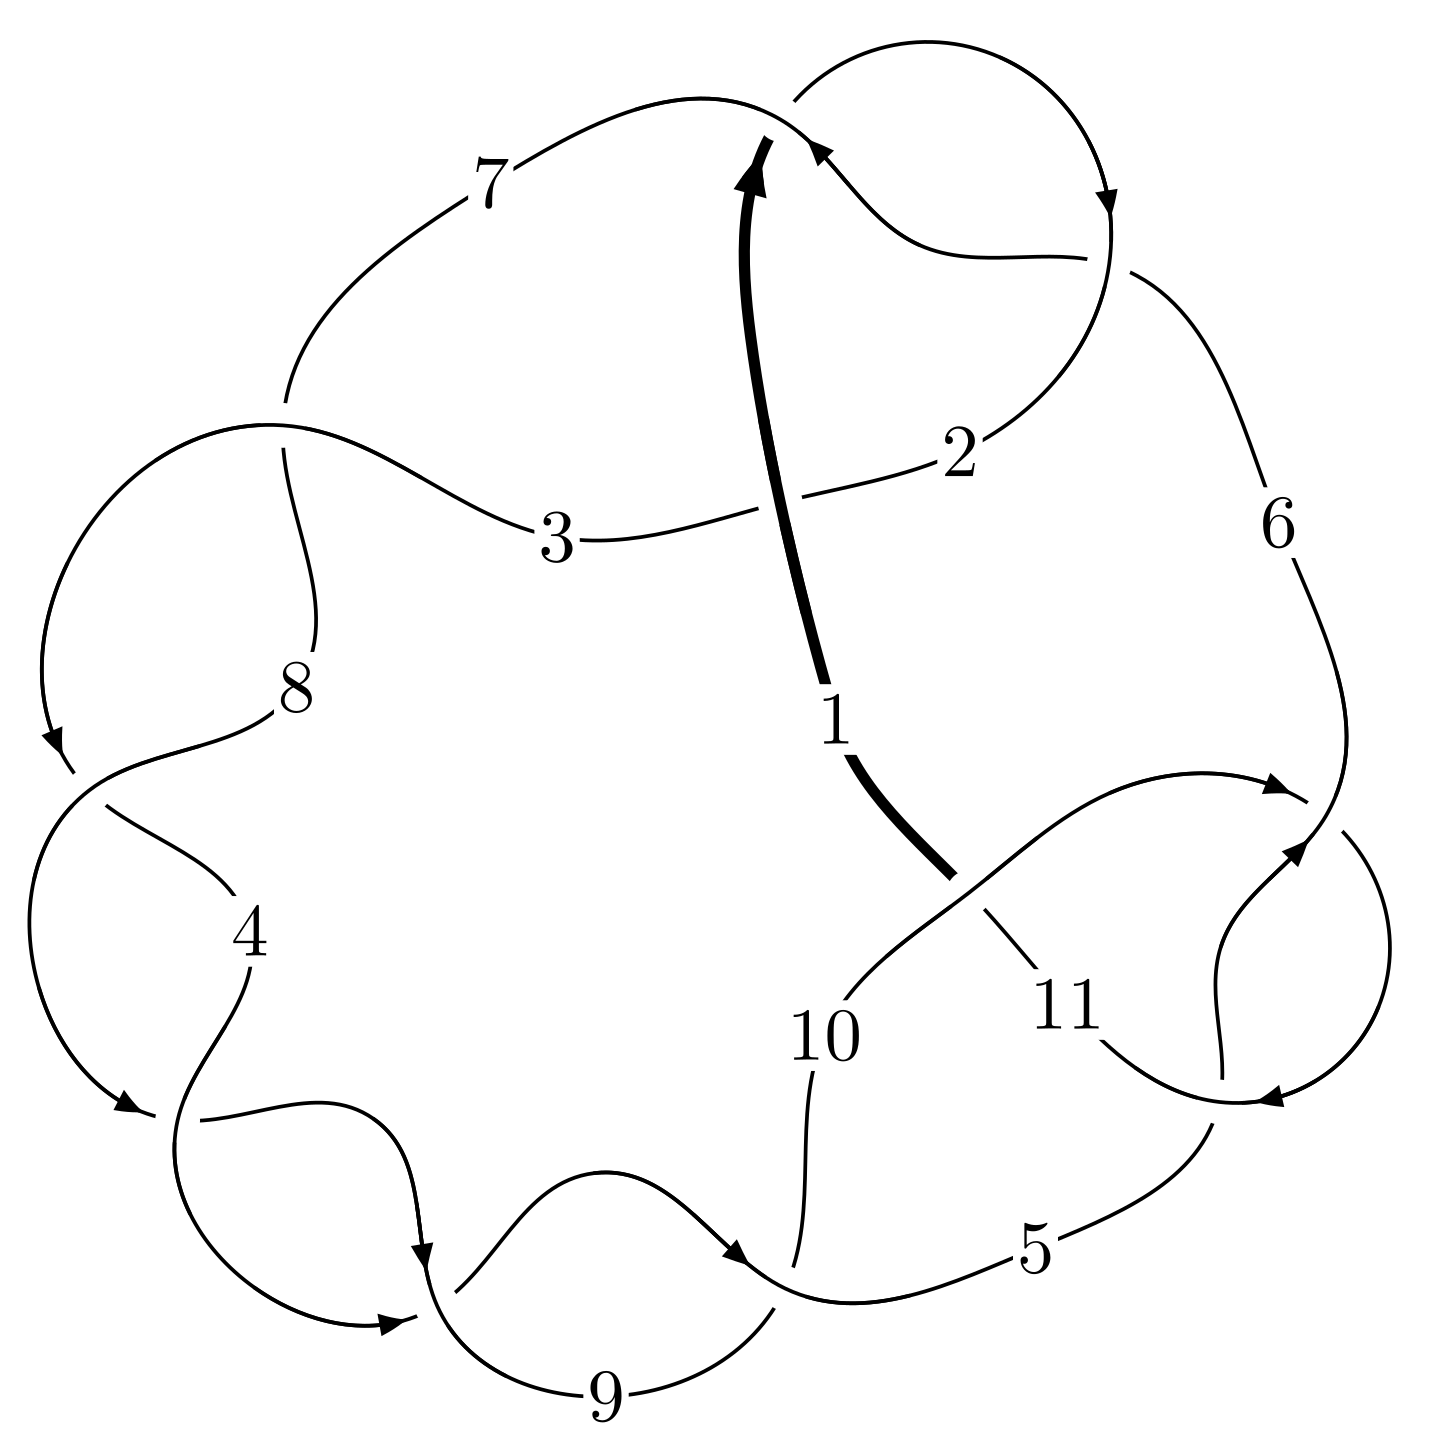
\includegraphics[width=112pt]{../../../GIT/diagram.site/Diagrams/png/428_11a_179.png}\\
\ \ \ A knot diagram\footnotemark}&
\allowdisplaybreaks
\textbf{Linearized knot diagam} \\
\cline{2-2}
 &
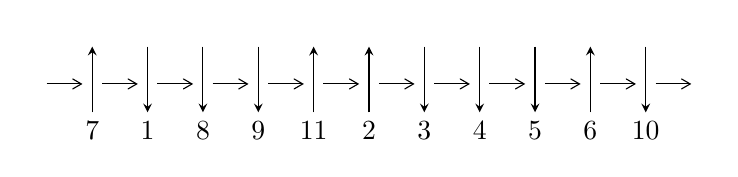
\begin{tikzpicture}[x=20pt, y=17pt]
	% nodes
	\node (C0) at (0, 0) {};
	\node (C1) at (1, 0) {};
	\node (C1U) at (1, +1) {};
	\node (C1D) at (1, -1) {7};

	\node (C2) at (2, 0) {};
	\node (C2U) at (2, +1) {};
	\node (C2D) at (2, -1) {1};

	\node (C3) at (3, 0) {};
	\node (C3U) at (3, +1) {};
	\node (C3D) at (3, -1) {8};

	\node (C4) at (4, 0) {};
	\node (C4U) at (4, +1) {};
	\node (C4D) at (4, -1) {9};

	\node (C5) at (5, 0) {};
	\node (C5U) at (5, +1) {};
	\node (C5D) at (5, -1) {11};

	\node (C6) at (6, 0) {};
	\node (C6U) at (6, +1) {};
	\node (C6D) at (6, -1) {2};

	\node (C7) at (7, 0) {};
	\node (C7U) at (7, +1) {};
	\node (C7D) at (7, -1) {3};

	\node (C8) at (8, 0) {};
	\node (C8U) at (8, +1) {};
	\node (C8D) at (8, -1) {4};

	\node (C9) at (9, 0) {};
	\node (C9U) at (9, +1) {};
	\node (C9D) at (9, -1) {5};

	\node (C10) at (10, 0) {};
	\node (C10U) at (10, +1) {};
	\node (C10D) at (10, -1) {6};

	\node (C11) at (11, 0) {};
	\node (C11U) at (11, +1) {};
	\node (C11D) at (11, -1) {10};
	\node (C12) at (12, 0) {};

	% arrows
	\draw[->,>={angle 60}]
	(C0) edge (C1) (C1) edge (C2) (C2) edge (C3) (C3) edge (C4) (C4) edge (C5) (C5) edge (C6) (C6) edge (C7) (C7) edge (C8) (C8) edge (C9) (C9) edge (C10) (C10) edge (C11) (C11) edge (C12) ;	\draw[->,>=stealth]
	(C1D) edge (C1U) (C2U) edge (C2D) (C3U) edge (C3D) (C4U) edge (C4D) (C5D) edge (C5U) (C6D) edge (C6U) (C7U) edge (C7D) (C8U) edge (C8D) (C9U) edge (C9D) (C10D) edge (C10U) (C11U) edge (C11D) ;
	\end{tikzpicture} \\
\hhline{~~} \\& 
\textbf{Solving Sequence} \\ \cline{2-2} 
 &
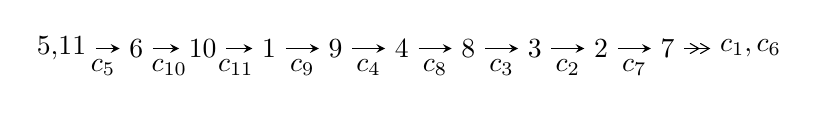
\begin{tikzpicture}[x=24pt, y=7pt]
	% node
	\node (A0) at (-1/8, 0) {5,11};
	\node (A1) at (1, 0) {6};
	\node (A2) at (2, 0) {10};
	\node (A3) at (3, 0) {1};
	\node (A4) at (4, 0) {9};
	\node (A5) at (5, 0) {4};
	\node (A6) at (6, 0) {8};
	\node (A7) at (7, 0) {3};
	\node (A8) at (8, 0) {2};
	\node (A9) at (9, 0) {7};
	\node (C1) at (1/2, -1) {$c_{5}$};
	\node (C2) at (3/2, -1) {$c_{10}$};
	\node (C3) at (5/2, -1) {$c_{11}$};
	\node (C4) at (7/2, -1) {$c_{9}$};
	\node (C5) at (9/2, -1) {$c_{4}$};
	\node (C6) at (11/2, -1) {$c_{8}$};
	\node (C7) at (13/2, -1) {$c_{3}$};
	\node (C8) at (15/2, -1) {$c_{2}$};
	\node (C9) at (17/2, -1) {$c_{7}$};
	\node (A10) at (41/4, 0) {$c_{1},c_{6}$};

	% edge
	\draw[->,>=stealth]	
	(A0) edge (A1) (A1) edge (A2) (A2) edge (A3) (A3) edge (A4) (A4) edge (A5) (A5) edge (A6) (A6) edge (A7) (A7) edge (A8) (A8) edge (A9) ;
	\draw[->>,>={angle 60}]	
	(A9) edge (A10);
\end{tikzpicture} \\ 

\end{tabular} \\

\footnotetext{
The image of knot diagram is generated by the software ``\textbf{Draw programme}" developed by Andrew Bartholomew(\url{http://www.layer8.co.uk/maths/draw/index.htm\#Running-draw}), where we modified some parts for our purpose(\url{https://github.com/CATsTAILs/LinksPainter}).
}\phantom \\ \newline 
\centering \textbf{Ideals for irreducible components\footnotemark of $X_{\text{par}}$} 
 
\begin{align*}
I^u_{1}&=\langle 
u^{10}+3 u^8+u^7+4 u^6+2 u^5+u^4+2 u^3- u^2-1\rangle \\
I^u_{2}&=\langle 
u^{18}- u^{17}+\cdots-2 u+1\rangle \\
\\
\end{align*}
\raggedright * 2 irreducible components of $\dim_{\mathbb{C}}=0$, with total 28 representations.\\
\footnotetext{All coefficients of polynomials are rational numbers. But the coefficients are sometimes approximated in decimal forms when there is not enough margin.}
\newpage
\renewcommand{\arraystretch}{1}
\centering \section*{I. $I^u_{1}= \langle u^{10}+3 u^8+u^7+4 u^6+2 u^5+u^4+2 u^3- u^2-1 \rangle$}
\flushleft \textbf{(i) Arc colorings}\\
\begin{tabular}{m{7pt} m{180pt} m{7pt} m{180pt} }
\flushright $a_{5}=$&$\begin{pmatrix}1\\0\end{pmatrix}$ \\
\flushright $a_{11}=$&$\begin{pmatrix}0\\u\end{pmatrix}$ \\
\flushright $a_{6}=$&$\begin{pmatrix}1\\- u^2\end{pmatrix}$ \\
\flushright $a_{10}=$&$\begin{pmatrix}- u\\u^3+u\end{pmatrix}$ \\
\flushright $a_{1}=$&$\begin{pmatrix}- u^3\\u^5+u^3+u\end{pmatrix}$ \\
\flushright $a_{9}=$&$\begin{pmatrix}u^3\\u^3+u\end{pmatrix}$ \\
\flushright $a_{4}=$&$\begin{pmatrix}- u^6- u^4+1\\- u^6-2 u^4- u^2\end{pmatrix}$ \\
\flushright $a_{8}=$&$\begin{pmatrix}- u^9-2 u^7- u^5+2 u^3+u\\- u^9-3 u^7-3 u^5+u\end{pmatrix}$ \\
\flushright $a_{3}=$&$\begin{pmatrix}- u^9- u^8-2 u^7-3 u^6-2 u^5-3 u^4+1\\- u^9- u^8-3 u^7-3 u^6-4 u^5-3 u^4-2 u^3+1\end{pmatrix}$ \\
\flushright $a_{2}=$&$\begin{pmatrix}- u^9- u^8-2 u^7-3 u^6-3 u^5-3 u^4+1\\- u^9- u^8-2 u^7-3 u^6-3 u^5-3 u^4- u^3+1\end{pmatrix}$ \\
\flushright $a_{7}=$&$\begin{pmatrix}- u^9+u^8-2 u^7+u^6- u^5+u^4+2 u^3- u^2+u\\- u^9+u^8-2 u^7+u^6- u^5+2 u^3-2 u^2+u-1\end{pmatrix}$\\ \flushright $a_{7}=$&$\begin{pmatrix}- u^9+u^8-2 u^7+u^6- u^5+u^4+2 u^3- u^2+u\\- u^9+u^8-2 u^7+u^6- u^5+2 u^3-2 u^2+u-1\end{pmatrix}$\\&\end{tabular}
\flushleft \textbf{(ii) Obstruction class $= -1$}\\~\\
\flushleft \textbf{(iii) Cusp Shapes $= -4 u^9+4 u^8-8 u^7+4 u^6-4 u^5+4 u^4+8 u^3-8 u^2+4 u-6$}\\~\\
\newpage\renewcommand{\arraystretch}{1}
\flushleft \textbf{(iv) u-Polynomials at the component}\newline \\
\begin{tabular}{m{50pt}|m{274pt}}
Crossings & \hspace{64pt}u-Polynomials at each crossing \\
\hline $$\begin{aligned}c_{1},c_{5},c_{6}\\c_{10}\end{aligned}$$&$\begin{aligned}
&u^{10}+3 u^8- u^7+4 u^6-2 u^5+u^4-2 u^3- u^2-1
\end{aligned}$\\
\hline $$\begin{aligned}c_{2},c_{11}\end{aligned}$$&$\begin{aligned}
&u^{10}+6 u^9+17 u^8+25 u^7+16 u^6-8 u^5-21 u^4-14 u^3- u^2+2 u+1
\end{aligned}$\\
\hline $$\begin{aligned}c_{3},c_{4},c_{7}\\c_{8},c_{9}\end{aligned}$$&$\begin{aligned}
&u^{10}-3 u^9-2 u^8+11 u^7- u^6-13 u^5+6 u^4+2 u^3-3 u^2+u-2
\end{aligned}$\\
\hline
\end{tabular}\\~\\
\newpage\renewcommand{\arraystretch}{1}
\flushleft \textbf{(v) Riley Polynomials at the component}\newline \\
\begin{tabular}{m{50pt}|m{274pt}}
Crossings & \hspace{64pt}Riley Polynomials at each crossing \\
\hline $$\begin{aligned}c_{1},c_{5},c_{6}\\c_{10}\end{aligned}$$&$\begin{aligned}
&y^{10}+6 y^9+17 y^8+25 y^7+16 y^6-8 y^5-21 y^4-14 y^3- y^2+2 y+1
\end{aligned}$\\
\hline $$\begin{aligned}c_{2},c_{11}\end{aligned}$$&$\begin{aligned}
&y^{10}-2 y^9+\cdots-6 y+1
\end{aligned}$\\
\hline $$\begin{aligned}c_{3},c_{4},c_{7}\\c_{8},c_{9}\end{aligned}$$&$\begin{aligned}
&y^{10}-13 y^9+\cdots+11 y+4
\end{aligned}$\\
\hline
\end{tabular}\\~\\
\newpage\flushleft \textbf{(vi) Complex Volumes and Cusp Shapes}
$$\begin{array}{c|c|c}  
\text{Solutions to }I^u_{1}& \I (\text{vol} + \sqrt{-1}CS) & \text{Cusp shape}\\
 \hline 
\begin{aligned}
u &= \phantom{-}0.405701 + 0.957098 I\end{aligned}
 & -2.02767 + 5.09588 I & -7.00928 - 9.34423 I \\ \hline\begin{aligned}
u &= \phantom{-}0.405701 - 0.957098 I\end{aligned}
 & -2.02767 - 5.09588 I & -7.00928 + 9.34423 I \\ \hline\begin{aligned}
u &= -0.928426\phantom{ +0.000000I}\end{aligned}
 & -11.5246\phantom{ +0.000000I} & -5.70350\phantom{ +0.000000I} \\ \hline\begin{aligned}
u &= -0.452669 + 1.159180 I\end{aligned}
 & -8.16772 - 8.20953 I & -10.99080 + 7.49201 I \\ \hline\begin{aligned}
u &= -0.452669 - 1.159180 I\end{aligned}
 & -8.16772 + 8.20953 I & -10.99080 - 7.49201 I \\ \hline\begin{aligned}
u &= -0.300956 + 0.659835 I\end{aligned}
 & \phantom{-}0.05290 - 1.41771 I & -1.07087 + 5.41263 I \\ \hline\begin{aligned}
u &= -0.300956 - 0.659835 I\end{aligned}
 & \phantom{-}0.05290 + 1.41771 I & -1.07087 - 5.41263 I \\ \hline\begin{aligned}
u &= \phantom{-}0.650332\phantom{ +0.000000I}\end{aligned}
 & -1.85975\phantom{ +0.000000I} & -4.37780\phantom{ +0.000000I} \\ \hline\begin{aligned}
u &= \phantom{-}0.486972 + 1.282400 I\end{aligned}
 & -19.3539 + 10.0674 I & -11.88841 - 5.78919 I \\ \hline\begin{aligned}
u &= \phantom{-}0.486972 - 1.282400 I\end{aligned}
 & -19.3539 - 10.0674 I & -11.88841 + 5.78919 I\\
 \hline 
 \end{array}$$\newpage\newpage\renewcommand{\arraystretch}{1}
\centering \section*{II. $I^u_{2}= \langle u^{18}- u^{17}+6 u^{16}-6 u^{15}+16 u^{14}-16 u^{13}+21 u^{12}-21 u^{11}+10 u^{10}-10 u^9-7 u^8+7 u^7-9 u^6+9 u^5- u^4+u^3+2 u^2-2 u+1 \rangle$}
\flushleft \textbf{(i) Arc colorings}\\
\begin{tabular}{m{7pt} m{180pt} m{7pt} m{180pt} }
\flushright $a_{5}=$&$\begin{pmatrix}1\\0\end{pmatrix}$ \\
\flushright $a_{11}=$&$\begin{pmatrix}0\\u\end{pmatrix}$ \\
\flushright $a_{6}=$&$\begin{pmatrix}1\\- u^2\end{pmatrix}$ \\
\flushright $a_{10}=$&$\begin{pmatrix}- u\\u^3+u\end{pmatrix}$ \\
\flushright $a_{1}=$&$\begin{pmatrix}- u^3\\u^5+u^3+u\end{pmatrix}$ \\
\flushright $a_{9}=$&$\begin{pmatrix}u^3\\u^3+u\end{pmatrix}$ \\
\flushright $a_{4}=$&$\begin{pmatrix}- u^6- u^4+1\\- u^6-2 u^4- u^2\end{pmatrix}$ \\
\flushright $a_{8}=$&$\begin{pmatrix}- u^9-2 u^7- u^5+2 u^3+u\\- u^9-3 u^7-3 u^5+u\end{pmatrix}$ \\
\flushright $a_{3}=$&$\begin{pmatrix}u^{12}+3 u^{10}+3 u^8-2 u^6-4 u^4- u^2+1\\u^{12}+4 u^{10}+6 u^8+2 u^6-3 u^4-2 u^2\end{pmatrix}$ \\
\flushright $a_{2}=$&$\begin{pmatrix}u^{16}+5 u^{14}+11 u^{12}+10 u^{10}- u^8-10 u^6-6 u^4- u+1\\-2 u^{17}+u^{16}+\cdots-3 u+2\end{pmatrix}$ \\
\flushright $a_{7}=$&$\begin{pmatrix}u^{15}+4 u^{13}+6 u^{11}-8 u^7-6 u^5+2 u^3+2 u\\u^{15}+5 u^{13}+10 u^{11}+7 u^9-4 u^7-8 u^5-2 u^3+u\end{pmatrix}$\\ \flushright $a_{7}=$&$\begin{pmatrix}u^{15}+4 u^{13}+6 u^{11}-8 u^7-6 u^5+2 u^3+2 u\\u^{15}+5 u^{13}+10 u^{11}+7 u^9-4 u^7-8 u^5-2 u^3+u\end{pmatrix}$\\&\end{tabular}
\flushleft \textbf{(ii) Obstruction class $= -1$}\\~\\
\flushleft \textbf{(iii) Cusp Shapes $= 4 u^{15}+20 u^{13}+40 u^{11}+24 u^9-28 u^7-44 u^5-4 u^3+12 u-10$}\\~\\
\newpage\renewcommand{\arraystretch}{1}
\flushleft \textbf{(iv) u-Polynomials at the component}\newline \\
\begin{tabular}{m{50pt}|m{274pt}}
Crossings & \hspace{64pt}u-Polynomials at each crossing \\
\hline $$\begin{aligned}c_{1},c_{5},c_{6}\\c_{10}\end{aligned}$$&$\begin{aligned}
&u^{18}+u^{17}+\cdots+2 u+1
\end{aligned}$\\
\hline $$\begin{aligned}c_{2},c_{11}\end{aligned}$$&$\begin{aligned}
&u^{18}+11 u^{17}+\cdots+6 u^2+1
\end{aligned}$\\
\hline $$\begin{aligned}c_{3},c_{4},c_{7}\\c_{8},c_{9}\end{aligned}$$&$\begin{aligned}
&(u^9+u^8-6 u^7-5 u^6+11 u^5+7 u^4-6 u^3-4 u^2- u+1)^2
\end{aligned}$\\
\hline
\end{tabular}\\~\\
\newpage\renewcommand{\arraystretch}{1}
\flushleft \textbf{(v) Riley Polynomials at the component}\newline \\
\begin{tabular}{m{50pt}|m{274pt}}
Crossings & \hspace{64pt}Riley Polynomials at each crossing \\
\hline $$\begin{aligned}c_{1},c_{5},c_{6}\\c_{10}\end{aligned}$$&$\begin{aligned}
&y^{18}+11 y^{17}+\cdots+6 y^2+1
\end{aligned}$\\
\hline $$\begin{aligned}c_{2},c_{11}\end{aligned}$$&$\begin{aligned}
&y^{18}-9 y^{17}+\cdots+12 y+1
\end{aligned}$\\
\hline $$\begin{aligned}c_{3},c_{4},c_{7}\\c_{8},c_{9}\end{aligned}$$&$\begin{aligned}
&(y^9-13 y^8+68 y^7-183 y^6+269 y^5-211 y^4+80 y^3-18 y^2+9 y-1)^{2}
\end{aligned}$\\
\hline
\end{tabular}\\~\\
\newpage\flushleft \textbf{(vi) Complex Volumes and Cusp Shapes}
$$\begin{array}{c|c|c}  
\text{Solutions to }I^u_{2}& \I (\text{vol} + \sqrt{-1}CS) & \text{Cusp shape}\\
 \hline 
\begin{aligned}
u &= \phantom{-}0.163695 + 1.039420 I\end{aligned}
 & -3.85110\phantom{ +0.000000I} & -13.61277 + 0. I\phantom{ +0.000000I} \\ \hline\begin{aligned}
u &= \phantom{-}0.163695 - 1.039420 I\end{aligned}
 & -3.85110\phantom{ +0.000000I} & -13.61277 + 0. I\phantom{ +0.000000I} \\ \hline\begin{aligned}
u &= \phantom{-}0.937573 + 0.014479 I\end{aligned}
 & -15.4587 - 4.9949 I & -8.86627 + 2.90812 I \\ \hline\begin{aligned}
u &= \phantom{-}0.937573 - 0.014479 I\end{aligned}
 & -15.4587 + 4.9949 I & -8.86627 - 2.90812 I \\ \hline\begin{aligned}
u &= -0.306317 + 0.859721 I\end{aligned}
 & -0.44198 - 1.55423 I & -2.94040 + 4.30527 I \\ \hline\begin{aligned}
u &= -0.306317 - 0.859721 I\end{aligned}
 & -0.44198 + 1.55423 I & -2.94040 - 4.30527 I \\ \hline\begin{aligned}
u &= \phantom{-}0.406229 + 1.141860 I\end{aligned}
 & -5.04794 + 3.86354 I & -8.03791 - 4.00946 I \\ \hline\begin{aligned}
u &= \phantom{-}0.406229 - 1.141860 I\end{aligned}
 & -5.04794 - 3.86354 I & -8.03791 + 4.00946 I \\ \hline\begin{aligned}
u &= -0.371894 + 1.189500 I\end{aligned}
 & -8.79106\phantom{ +0.000000I} & -12.57530 + 0. I\phantom{ +0.000000I} \\ \hline\begin{aligned}
u &= -0.371894 - 1.189500 I\end{aligned}
 & -8.79106\phantom{ +0.000000I} & -12.57530 + 0. I\phantom{ +0.000000I} \\ \hline\begin{aligned}
u &= -0.734633 + 0.083595 I\end{aligned}
 & -5.04794 + 3.86354 I & -8.03791 - 4.00946 I \\ \hline\begin{aligned}
u &= -0.734633 - 0.083595 I\end{aligned}
 & -5.04794 - 3.86354 I & -8.03791 + 4.00946 I \\ \hline\begin{aligned}
u &= -0.476691 + 1.280860 I\end{aligned}
 & -15.4587 - 4.9949 I & -8.86627 + 2.90812 I \\ \hline\begin{aligned}
u &= -0.476691 - 1.280860 I\end{aligned}
 & -15.4587 + 4.9949 I & -8.86627 - 2.90812 I \\ \hline\begin{aligned}
u &= \phantom{-}0.470193 + 1.289670 I\end{aligned}
 & -19.4826\phantom{ +0.000000I} & -12.12278 + 0. I\phantom{ +0.000000I} \\ \hline\begin{aligned}
u &= \phantom{-}0.470193 - 1.289670 I\end{aligned}
 & -19.4826\phantom{ +0.000000I} & -12.12278 + 0. I\phantom{ +0.000000I} \\ \hline\begin{aligned}
u &= \phantom{-}0.411845 + 0.333652 I\end{aligned}
 & -0.44198 - 1.55423 I & -2.94040 + 4.30527 I \\ \hline\begin{aligned}
u &= \phantom{-}0.411845 - 0.333652 I\end{aligned}
 & -0.44198 + 1.55423 I & -2.94040 - 4.30527 I\\
 \hline 
 \end{array}$$\newpage
\newpage\renewcommand{\arraystretch}{1}
\centering \section*{ III. u-Polynomials}
\begin{tabular}{m{50pt}|m{274pt}}
Crossings & \hspace{64pt}u-Polynomials at each crossing \\
\hline $$\begin{aligned}c_{1},c_{5},c_{6}\\c_{10}\end{aligned}$$&$\begin{aligned}
&(u^{10}+3 u^8+\cdots- u^2-1)(u^{18}+u^{17}+\cdots+2 u+1)
\end{aligned}$\\
\hline $$\begin{aligned}c_{2},c_{11}\end{aligned}$$&$\begin{aligned}
&(u^{10}+6 u^9+17 u^8+25 u^7+16 u^6-8 u^5-21 u^4-14 u^3- u^2+2 u+1)\\
&\cdot(u^{18}+11 u^{17}+\cdots+6 u^2+1)
\end{aligned}$\\
\hline $$\begin{aligned}c_{3},c_{4},c_{7}\\c_{8},c_{9}\end{aligned}$$&$\begin{aligned}
&(u^9+u^8-6 u^7-5 u^6+11 u^5+7 u^4-6 u^3-4 u^2- u+1)^2\\
&\cdot(u^{10}-3 u^9-2 u^8+11 u^7- u^6-13 u^5+6 u^4+2 u^3-3 u^2+u-2)
\end{aligned}$\\
\hline
\end{tabular}\newpage\renewcommand{\arraystretch}{1}
\centering \section*{ IV. Riley Polynomials}
\begin{tabular}{m{50pt}|m{274pt}}
Crossings & \hspace{64pt}Riley Polynomials at each crossing \\
\hline $$\begin{aligned}c_{1},c_{5},c_{6}\\c_{10}\end{aligned}$$&$\begin{aligned}
&(y^{10}+6 y^9+17 y^8+25 y^7+16 y^6-8 y^5-21 y^4-14 y^3- y^2+2 y+1)\\
&\cdot(y^{18}+11 y^{17}+\cdots+6 y^2+1)
\end{aligned}$\\
\hline $$\begin{aligned}c_{2},c_{11}\end{aligned}$$&$\begin{aligned}
&(y^{10}-2 y^9+\cdots-6 y+1)(y^{18}-9 y^{17}+\cdots+12 y+1)
\end{aligned}$\\
\hline $$\begin{aligned}c_{3},c_{4},c_{7}\\c_{8},c_{9}\end{aligned}$$&$\begin{aligned}
&(y^9-13 y^8+68 y^7-183 y^6+269 y^5-211 y^4+80 y^3-18 y^2+9 y-1)^{2}\\
&\cdot(y^{10}-13 y^9+\cdots+11 y+4)
\end{aligned}$\\
\hline
\end{tabular}
\vskip 2pc
\end{document}